\documentclass{article}%
\usepackage[T1]{fontenc}%
\usepackage[utf8]{inputenc}%
\usepackage{lmodern}%
\usepackage{textcomp}%
\usepackage{lastpage}%
\usepackage{authblk}%
\usepackage{graphicx}%
%
\title{Hemin{-}Induced Modifications of the Antigenicity and Hemin{-}Binding Capacity of Porphyromonas gingivalis Lipopolysaccharide}%
\author{Mary Cook}%
\affil{National Creative Research Initiatives Center for Nuclear Receptor Signals, Hormone Research Center, School of Biological Sciences and Technology, Chonnam National University, Gwangju, Republic of Korea}%
\date{01{-}01{-}2014}%
%
\begin{document}%
\normalsize%
\maketitle%
\section{Abstract}%
\label{sec:Abstract}%
The Monitor has received a report that Sharen B Squristin an Illinois chemical engineer was arrested in San Diego City Jail on charges of manufacturing unapproved pharmaceuticals with fraud and forging prescriptions to obtain a controlled substance.\newline%
According to the case report, Squristin is charged with 27 counts, including one count of evading a prescription to obtain illegal pharmaceuticals with fraud and an additional count of bank fraud. Squristin was released from the Butte County Jail just before 1 p.m. on Monday.\newline%
The trial is expected to begin in March.\newline%
The findings of this investigation were conducted by State Sen. Neil Derry, D{-}Burbank, and the City of San Diegos Investigative Liaison Unit.\newline%
The Los Angeles Times initially reported that Squristin had been arrested following an inquiry by the Fraud Research Section of the Consumer Fraud and Counterfeit Enforcement Center. According to the Times report, Squristin is alleged to have made fraudulent prescription purchases through a web of companies, brokerage accounts and open posts on a fake blog.\newline%
Under California law, the federal government issues designated qualified outpatient prescriptions to qualified physicians. These prescriptions are primarily given to cancer patients to manage other illnesses.\newline%
According to the Times report, more than 20 hospitals and doctors offices received orders from the fraud laboratory, and the majority of the prescriptions included nausea, vomiting, gas and diarrhea.\newline%
Specifically, the experiments tested were conducted on cancer cells living in the patients body and found that they were an interactions of chemical signals that could be induced by its chemical formula and triggered by its endocrine system.\newline%
According to the Times report, Squristins lab is believed to have manufactured more than \$100,000 worth of fraudulent prescription drugs.\newline%
The Los Angeles Times story notes that California State Senator Derry responded to public criticism of the investigation by saying it is important to bring the fraud cases to light so that Californians may understand the financial practices being used in the prescription drug industry.

%
\subsection{Image Analysis}%
\label{subsec:ImageAnalysis}%


\begin{figure}[h!]%
\centering%
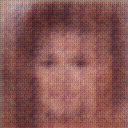
\includegraphics[width=150px]{500_fake_images/samples_5_6.png}%
\caption{A Man Is Wearing A Tie And A Hat}%
\end{figure}

%
\end{document}